% =====================================================================
%  Urban Track  |  Global project documentation
%  Final delivery dossier - built with pdfLaTeX
%
%  Visual identity: this document uses the exact colour palette of the
%  Urban Track website (templates/base.html, tailwind.config):
%    military green  #5C6B2F (dominant)
%    accent pink     #EC4899 (call to action)
%    charcoal        #1C1C1B (text)
%    white / off-white surfaces
% =====================================================================
\documentclass[11pt,a4paper]{article}

% ---------------------------------------------------------------------
%  Fonts & typography
% ---------------------------------------------------------------------
\usepackage[T1]{fontenc}
\usepackage[utf8]{inputenc}
\usepackage{tgheros}
\usepackage{tgcursor}
\renewcommand{\familydefault}{\sfdefault}
\usepackage[english]{babel}
\usepackage{microtype}
\usepackage[a4paper,top=2.5cm,bottom=2.4cm,left=2.3cm,right=2.3cm,headheight=22pt]{geometry}

% ---------------------------------------------------------------------
%  Palette - exact website tokens
% ---------------------------------------------------------------------
\usepackage{xcolor}
\definecolor{mil50}{HTML}{F2F4EC}
\definecolor{mil100}{HTML}{E1E6CF}
\definecolor{mil300}{HTML}{A9B57A}
\definecolor{mil500}{HTML}{5C6B2F}
\definecolor{mil700}{HTML}{3F4A20}
\definecolor{mil900}{HTML}{2A3116}

\definecolor{acc50}{HTML}{FDF2F8}
\definecolor{acc300}{HTML}{F9A8D4}
\definecolor{acc500}{HTML}{EC4899}
\definecolor{acc700}{HTML}{BE185D}

\definecolor{char50}{HTML}{F5F5F4}
\definecolor{char300}{HTML}{A8A8A6}
\definecolor{char700}{HTML}{3F3F3E}
\definecolor{char900}{HTML}{1C1C1B}

% Semantic status colours taken from the website badges
\definecolor{okred}{HTML}{B91C1C}

% ---------------------------------------------------------------------
%  Packages
% ---------------------------------------------------------------------
\usepackage{graphicx}
\usepackage{xcolor}
\usepackage{amsmath,amssymb}
\usepackage{array}
\usepackage{tabularx}
\usepackage{booktabs}
\usepackage{longtable}
\usepackage{colortbl}
\usepackage{multirow}
\usepackage{enumitem}
\usepackage{fancyhdr}
\usepackage{titlesec}
\usepackage{tocloft}
\usepackage{lastpage}
\usepackage{listings}
\usepackage{seqsplit}
\usepackage{tikz}
\usetikzlibrary{arrows.meta,positioning,calc,shapes.geometric,fit,backgrounds}
\usepackage[most]{tcolorbox}
\usepackage[hidelinks]{hyperref}

\graphicspath{{../static/img/}{static/img/}{./}}

% ---------------------------------------------------------------------
%  Hyperlinks
% ---------------------------------------------------------------------
\hypersetup{
  colorlinks=true,
  linkcolor=mil700,
  urlcolor=acc700,
  citecolor=mil700,
  pdftitle={Urban Track - Global Project Documentation},
  pdfauthor={Urban Track Engineering},
  pdfsubject={Final delivery dossier},
  pdfkeywords={Urban Track, Django, certification, urban development, Africa}
}
\urlstyle{same}

% ---------------------------------------------------------------------
%  Global layout
% ---------------------------------------------------------------------
\setlength{\parindent}{0pt}
\setlength{\parskip}{6pt}
\renewcommand{\arraystretch}{1.25}
\raggedbottom
\setlength{\emergencystretch}{2em}

% ---------------------------------------------------------------------
%  Headers & footers
% ---------------------------------------------------------------------
\pagestyle{fancy}
\fancyhf{}
\fancyhead[L]{\small\textcolor{char700}{\textbf{Urban Track}}}
\fancyhead[R]{\small\textcolor{char700}{Global project documentation}}
\fancyfoot[L]{\small\textcolor{char300}{Final delivery \textbullet\ November 2026}}
\fancyfoot[R]{\small\textcolor{mil700}{\textbf{\thepage}\,/\,\pageref{LastPage}}}
\renewcommand{\headrulewidth}{0.4pt}
\renewcommand{\headrule}{\hbox to\headwidth{\color{mil300}\leaders\hrule height \headrulewidth\hfill}}
\renewcommand{\footrulewidth}{0pt}
\fancypagestyle{plain}{
  \fancyhf{}
  \fancyfoot[L]{\small\textcolor{char300}{Final delivery \textbullet\ November 2026}}
  \fancyfoot[R]{\small\textcolor{mil700}{\textbf{\thepage}\,/\,\pageref{LastPage}}}
  \renewcommand{\headrulewidth}{0pt}
}

% ---------------------------------------------------------------------
%  Section styling
% ---------------------------------------------------------------------
\titleformat{\section}
  {\Large\bfseries\color{mil700}}
  {\thesection}{0.7em}{}
  [{\vspace{0.25em}\color{acc500}\titlerule[1.1pt]}]
\titleformat{\subsection}
  {\large\bfseries\color{char900}}
  {\thesubsection}{0.6em}{}
\titleformat{\subsubsection}
  {\normalsize\bfseries\color{mil700}}
  {\thesubsubsection}{0.5em}{}
\titlespacing*{\section}{0pt}{1.8ex plus 1ex minus .2ex}{1.0ex}
\titlespacing*{\subsection}{0pt}{1.4ex plus .8ex minus .2ex}{0.6ex}

% ---------------------------------------------------------------------
%  Table of contents styling
% ---------------------------------------------------------------------
\renewcommand{\contentsname}{Table of contents}
\renewcommand{\cfttoctitlefont}{\Huge\bfseries\color{mil700}}
\renewcommand{\cftaftertoctitle}{\hfill}
\renewcommand{\cftsecfont}{\color{char900}\bfseries}
\renewcommand{\cftsecpagefont}{\color{mil700}\bfseries}
\renewcommand{\cftsubsecfont}{\color{char700}}
\renewcommand{\cftsubsecpagefont}{\color{mil500}}
\setlength{\cftbeforesecskip}{5pt}
\setlength{\cftbeforesubsecskip}{2pt}

% ---------------------------------------------------------------------
%  Table helpers
% ---------------------------------------------------------------------
\newcolumntype{L}[1]{>{\raggedright\arraybackslash}p{#1}}
\newcolumntype{Y}{>{\raggedright\arraybackslash}X}
\newcommand{\splittt}[1]{{\ttfamily\seqsplit{#1}}}
\newcommand{\theadcell}[1]{\textcolor{white}{\textbf{#1}}}
\newcommand{\tablehead}[1]{\rowcolor{mil900}#1}
\newcommand{\tablealt}{\rowcolor{mil50}}

% ---------------------------------------------------------------------
%  Callout boxes
% ---------------------------------------------------------------------
\newtcolorbox{keybox}[1][]{
  enhanced, breakable, colback=mil50, colframe=mil500,
  boxrule=0pt, leftrule=3pt, arc=2pt, left=8pt, right=8pt,
  top=6pt, bottom=6pt, #1
}
\newtcolorbox{accentbox}[1][]{
  enhanced, breakable, colback=acc50, colframe=acc500,
  boxrule=0pt, leftrule=3pt, arc=2pt, left=8pt, right=8pt,
  top=6pt, bottom=6pt, #1
}
\newtcolorbox{notebox}[1][]{
  enhanced, breakable, colback=char50, colframe=char300,
  boxrule=0pt, leftrule=3pt, arc=2pt, left=8pt, right=8pt,
  top=6pt, bottom=6pt, #1
}
\newtcolorbox{dangerbox}[1][]{
  enhanced, breakable, colback=red!4, colframe=okred,
  boxrule=0pt, leftrule=3pt, arc=2pt, left=8pt, right=8pt,
  top=6pt, bottom=6pt, #1
}

% ---------------------------------------------------------------------
%  Status chips
% ---------------------------------------------------------------------
\newcommand{\chip}[2]{%
  \tikz[baseline=-0.6ex]{\node[rounded corners=2pt, inner sep=2.5pt,
    fill=#1, text=white, font=\scriptsize\bfseries]{#2};}%
}
\newcommand{\delivered}{\chip{mil500}{DELIVERED}}
\newcommand{\partiald}{\chip{acc500}{PARTIAL}}
\newcommand{\planned}{\chip{char700}{PLANNED}}
\newcommand{\pending}{\chip{acc700}{PENDING}}

% ---------------------------------------------------------------------
%  Stat card
% ---------------------------------------------------------------------
\newcommand{\statbox}[2]{%
  \begin{minipage}[t]{0.155\textwidth}
    \centering
    {\fontsize{23}{25}\selectfont\bfseries\color{mil700}#1}\\[3pt]
    {\scriptsize\color{char300}\MakeUppercase{#2}}
  \end{minipage}%
}

% ---------------------------------------------------------------------
%  Code listings
% ---------------------------------------------------------------------
\lstdefinestyle{ut}{
  backgroundcolor=\color{char50},
  basicstyle=\ttfamily\small\color{char900},
  keywordstyle=\color{mil700}\bfseries,
  commentstyle=\color{char300}\itshape,
  stringstyle=\color{acc700},
  numberstyle=\tiny\color{char300},
  frame=single,
  rulecolor=\color{char300},
  breaklines=true,
  breakatwhitespace=false,
  columns=fullflexible,
  keepspaces=true,
  showstringspaces=false,
  xleftmargin=6pt,
  xrightmargin=6pt,
  aboveskip=8pt,
  belowskip=8pt,
}
\lstset{style=ut}

% =====================================================================
\begin{document}

% ---------------------------------------------------------------------
%  TITLE PAGE
% ---------------------------------------------------------------------
\begin{titlepage}
\thispagestyle{empty}
\noindent
\begin{tcolorbox}[enhanced, colback=mil900, colframe=mil900, boxrule=0pt,
  arc=0pt, width=\textwidth, left=1.1cm, right=1.1cm, top=1.2cm, bottom=1.4cm]
  \color{white}
  
\includegraphics[width=6.2cm]{logo_large_white.png}\\[1.5cm]
  {\color{acc300}\bfseries\large GLOBAL PROJECT DOCUMENTATION}\\[0.45cm]
  {\fontsize{40}{46}\selectfont\bfseries Urban Track}\\[0.45cm]
  {\Large The trust layer of urban development in Africa}\\[0.2cm]
  {\large Cross-verified experience, permanent professional identity and certified CVs}
  \vspace{0.85cm}

  {\color{mil100}\small Python 3.12 \textbullet\ Django 6.1 \textbullet\ SQLite
   \textbullet\ Tailwind CSS \textbullet\ WeasyPrint}
\end{tcolorbox}

\vspace{0.9cm}
{\color{mil700}\bfseries\Large Final delivery dossier}\\[0.15cm]
{\color{char700}\large Version 1.0 \textbullet\ November 2026}

\vspace{0.45cm}
\noindent
\begin{minipage}[c]{0.24\textwidth}
  
\includegraphics[width=\linewidth]{cga_logo.png}
\end{minipage}\hfill
\begin{minipage}[c]{0.72\textwidth}
  \raggedleft
  {\color{mil700}\bfseries\large Prepared by CGA}\\[2pt]
  {\color{char700}March 2026 -- October 2026}
\end{minipage}

\vfill

\renewcommand{\arraystretch}{1.5}
\begin{tabularx}{\textwidth}{@{}>{\bfseries\color{mil700}}l Y@{}}
  \toprule
  Document & Global project documentation \\
  Version & 1.0: final delivery \\
  Date & November 2026 \\
  Prepared by & CGA \\
  Project period & March 2026 -- October 2026 \\
  Status & Final \\
  Audience & Client, project sponsors, technical evaluators \\
  Product & Urban Track: trust layer for urban development \\
  Repository & \texttt{UrbanTrack}: Django modular monolith \\
  Classification & Delivery dossier \\
  \bottomrule
\end{tabularx}

\end{titlepage}

% ---------------------------------------------------------------------
%  FRONT MATTER
% ---------------------------------------------------------------------
\clearpage
\pagenumbering{roman}
\tableofcontents
\clearpage
\pagenumbering{arabic}

% =====================================================================
\section{Executive summary}
% =====================================================================

Urban Track is a trust layer for the African urban development sector. It
replaces unverifiable self-declared CVs with \textbf{cross-confirmed
professional experience}: a company publishes the projects it actually carried
out and declares the experts who contributed; each expert personally confirms,
adjusts or rejects the declaration. Only experience confirmed by both parties
is certified, displayed on public profiles and exported into donor-ready CVs.

The platform is a production-structured \textbf{Django 6.1 modular monolith}.
The delivered scope covers the complete certification workflow, expert
identity and portfolios, project publishing with donor-format metadata, a
two-skin bilingual CV generator with PDF and Word export, a job board with
application decisions and reminders, a system administration panel, branded
transactional email, structured audit logging, and a CI/CD pipeline.

\begin{center}
  \statbox{6}{application modules}
  \hfill
  \statbox{22}{data models}
  \hfill
  \statbox{66}{application routes}
  \hfill
  \statbox{66}{HTML templates}
  \hfill
  \statbox{288}{automated tests}
  \hfill
  \statbox{80\%}{CI coverage gate}
\end{center}

\begin{keybox}
\textbf{The single message of this delivery.} Urban Track is functional
end-to-end today: a user can sign up, obtain a permanent \texttt{OX-XXXXXX}
identity, publish or join a project, get a contribution independently
confirmed, see it certified on a public profile, export it as a professional CV
and apply to or publish a mission: with every step traceable and auditable.
\end{keybox}

\subsection*{Delivered outcomes at a glance}

\begin{itemize}[leftmargin=1.4em,itemsep=3pt]
  \item \textbf{Identity that lasts.} Every account receives a free, permanent,
        unique professional identifier in the \texttt{OX-XXXXXX} format, usable
        as a public URL and on printed CVs.
  \item \textbf{Certification that cannot be self-granted.} A contribution only
        becomes certified after the named expert personally validates the
        company's declaration, or after the client counter-signs an independent
        consultant's role.
  \item \textbf{Certified data that cannot be silently altered.} Once confirmed,
        the protected fields of a contribution are immutable; any change
        restarts a complete validation cycle.
  \item \textbf{CVs aligned with donor expectations.} Two professional skins
        (AFD and World Bank), French and English labels, certified experience
        visually separated from self-declared sections, and PDF/Word export.
  \item \textbf{A working marketplace.} Job offers, cover letters,
        accept/decline decisions, notifications and deadline reminders are
        implemented and tested.
  \item \textbf{Operational maturity.} Environment-driven settings, structured
        logging with request correlation, audit events, dependency security
        auditing, automated tests and a VPS deployment workflow.
\end{itemize}

\begin{notebox}
\textbf{Reading guide.} Sections~\ref{sec:context}--\ref{sec:workflow}
describe the product and its business rules. Sections~\ref{sec:architecture}--\ref{sec:data}
describe how it is built. Sections~\ref{sec:security}--\ref{sec:ops} describe
how it is secured, tested and operated. Section~\ref{sec:status} states exactly
what is delivered versus what remains planned, and Section~\ref{sec:start}
is the developer quick-start.
\end{notebox}

% =====================================================================
\section{Context and vision}
\label{sec:context}
% =====================================================================

\subsection{The problem}

In African urban development, hiring and partnership decisions too often rest
on CVs that cannot be checked. References are rarely followed up, individual
contributors disappear behind institutional signatures, and funders
(World Bank, AFD, European Union, national agencies) keep their own siloed
records. The consequences are concrete:

\begin{itemize}[leftmargin=1.4em,itemsep=3pt]
  \item hours lost searching for qualified consultants;
  \item hiring mistakes caused by unverifiable expertise;
  \item credit that never reaches the professionals who actually delivered the work.
\end{itemize}

\subsection{The solution}

Urban Track applies the co-author logic of academic publishing to the urban
sector. The company that carried out a project publishes it and declares its
contributors; each contributor is asked to confirm the declaration. The
platform is therefore not a CV-hosting website: it is a \textbf{verification
protocol} with a public, traceable output.

\begin{center}
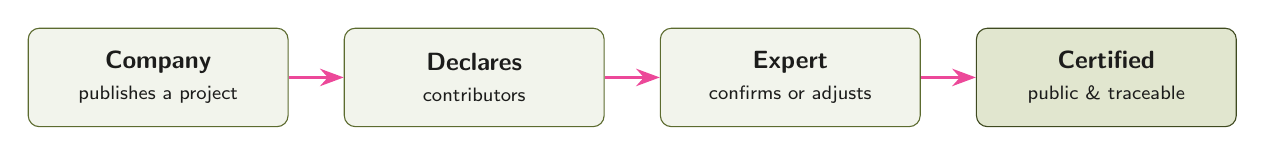
\begin{tikzpicture}[
  box/.style={draw=mil500, fill=mil50, rounded corners=4pt, minimum width=3.3cm,
    minimum height=1.25cm, align=center, font=\small\bfseries, text=char900},
  arr/.style={-{Stealth[length=3mm,width=2.2mm]}, draw=acc500, line width=1.2pt},
  node distance=0.7cm
]
  \node[box] (company) {Company\\{\scriptsize\mdseries publishes a project}};
  \node[box, right=of company] (declare) {Declares\\{\scriptsize\mdseries contributors}};
  \node[box, right=of declare] (confirm) {Expert\\{\scriptsize\mdseries confirms or adjusts}};
  \node[box, right=of confirm, fill=mil100, draw=mil700] (certify) {Certified\\{\scriptsize\mdseries public \& traceable}};
  \draw[arr] (company) -- (declare);
  \draw[arr] (declare) -- (confirm);
  \draw[arr] (confirm) -- (certify);
\end{tikzpicture}
\end{center}

\subsection{Value proposition by audience}

\begin{center}
\renewcommand{\arraystretch}{1.35}
\begin{tabularx}{\textwidth}{@{}L{3.4cm}Y@{}}
  \toprule
  \tablehead{\theadcell{Audience} & \theadcell{Value delivered}} \\
  \midrule
  \textbf{Individual experts} &
  A free account, a permanent professional identity, a public profile centred
  on certified experience, and donor-ready CVs in French and English. \\
  \tablealt
  \textbf{Engineering firms and consultancies} &
  Publish verified references, build certified teams and recruit on traceable
  track records rather than on claims. \\
  \textbf{Funders and public institutions} &
  A clearer trust base for partners and suppliers, with declarations traceable
  to projects and contributors. \\
  \bottomrule
\end{tabularx}
\end{center}

\subsection{Guiding business invariants}

These rules are not guidelines: they are enforced in services, model
\texttt{save()} methods and database constraints.

\begin{enumerate}[leftmargin=1.8em,itemsep=4pt]
  \item \textbf{Certification comes only from independent cross-confirmation.}
        A company declares, the expert personally validates.
  \item \textbf{Adjusting wording re-triggers validation.} A modified
        contribution must be re-validated by the company.
  \item \textbf{Existing accounts are linked, never duplicated.} An invited
        email that matches an account is attached to that account.
  \item \textbf{Reminders are capped.} At most two automatic reminders, after
        which the invitation expires (about 14 days).
  \item \textbf{Humans intervene only for arbitration.} Administrative action
        is reserved for disputes.
  \item \textbf{Certified data is immutable.} Protected fields cannot change
        without a new validation cycle.
  \item \textbf{Public traceability survives privacy changes.} A private,
        draft or archived project that holds a certified contribution keeps a
        minimal public proof page (name, client, dates, certified contributors).
\end{enumerate}

% =====================================================================
\section{Actors, roles and identity}
\label{sec:actors}
% =====================================================================

\subsection{Account types}

The custom user model deliberately separates the \emph{account role} from the
\emph{professional relationship} to an organisation.

\begin{center}
\renewcommand{\arraystretch}{1.35}
\begin{tabularx}{\textwidth}{@{}L{3.2cm}Y@{}}
  \toprule
  \tablehead{\theadcell{Account type} & \theadcell{Capabilities}} \\
  \midrule
  \textbf{User (expert)} &
  The default account. Any user can publish projects, declare contributors,
  confirm their own contributions, maintain a public portfolio, generate CVs,
  publish job offers and apply to missions. \\
  \tablealt
  \textbf{Administrator (nominated)} &
  A privileged account nominated by a superuser. It can access the
  \texttt{/admin-panel/} operational console: user management, project and job
  supervision, application overview. \\
  \textbf{Superuser} &
  Django's technical administrator. Has full access, including the native
  Django admin and dispute-arbitration actions. \\
  \bottomrule
\end{tabularx}
\end{center}

\subsection{The permanent professional identity}

At first save, every user receives a professional identifier formatted
\texttt{OX-XXXXXX}. It is:

\begin{itemize}[leftmargin=1.4em,itemsep=3pt]
  \item \textbf{permanent}: generated once and never modified;
  \item \textbf{unique}: enforced by a database unique constraint, with a
        pre-save collision check and a retry budget;
  \item \textbf{readable}: alphabet stripped of ambiguous characters
        (\texttt{I}, \texttt{O}, \texttt{0}, \texttt{1});
  \item \textbf{publicly usable}: the expert profile URL is anchored on it,
        e.g.\ \texttt{/experts/OX-XXXXXX/}.
\end{itemize}

\subsection{Company membership lifecycle (T2)}

Joining an existing company is never implicit. The only ways in are: the
founder's approved membership at company creation, a request approved by a
company administrator, or an administrator invitation accepted by the user.
\texttt{User.company} is populated only for approved members, so public pages
never leak a pending affiliation.

\begin{center}
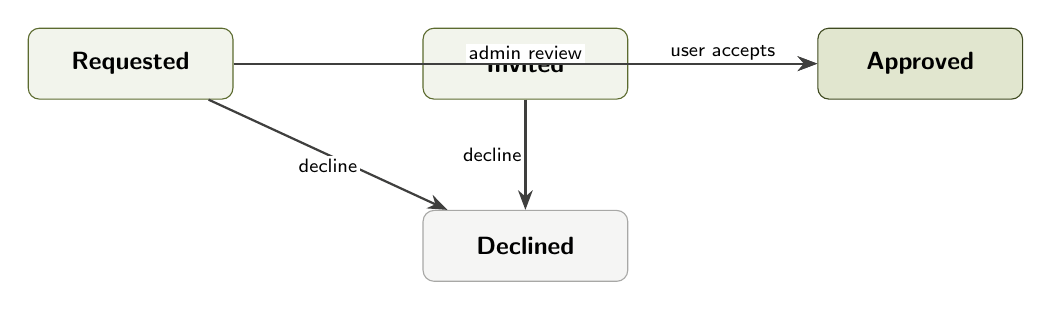
\begin{tikzpicture}[
  st/.style={draw=mil500, fill=mil50, rounded corners=4pt, minimum width=2.6cm,
    minimum height=0.9cm, align=center, font=\small\bfseries},
  done/.style={draw=mil700, fill=mil100, rounded corners=4pt, minimum width=2.6cm,
    minimum height=0.9cm, align=center, font=\small\bfseries},
  off/.style={draw=char300, fill=char50, rounded corners=4pt, minimum width=2.6cm,
    minimum height=0.9cm, align=center, font=\small\bfseries},
  arr/.style={-{Stealth[length=2.5mm]}, draw=char700, line width=0.8pt},
  lab/.style={font=\scriptsize, fill=white, inner sep=1pt}
]
  \node[st] (req) {Requested};
  \node[st, right=2.4cm of req] (inv) {Invited};
  \node[done, right=2.4cm of inv] (appr) {Approved};
  \node[off, below=1.4cm of inv] (decl) {Declined};
  \draw[arr] (req) -- node[above,lab]{admin review} (appr);
  \draw[arr] (inv) -- node[above,lab]{user accepts} (appr);
  \draw[arr] (req) -- node[below,lab]{decline} (decl);
  \draw[arr] (inv) -- node[left,lab]{decline} (decl);
\end{tikzpicture}
\end{center}

Every review stores \texttt{reviewed\_by} and \texttt{reviewed\_at} for audit.
The same approved company is what appears on project declarations, public
company pages and job offers.

% =====================================================================
\section{Functional scope}
\label{sec:functions}
% =====================================================================

The application is divided into six cohesive Django modules plus the project
configuration module. Each module owns one business capability and exposes its
state transitions through services rather than through ad-hoc view code.

\begin{center}
\renewcommand{\arraystretch}{1.35}
\begin{tabularx}{\textwidth}{@{}L{3.1cm}Y@{}}
  \toprule
  \tablehead{\theadcell{Module} & \theadcell{Responsibility}} \\
  \midrule
  \texttt{accounts} & Identity, permanent OX-ID, authentication, email
  confirmation, company memberships, expert portfolio and public profiles,
  expert directory. \\
  \tablealt
  \texttt{projects} & Project model and lifecycle, donor-format referentials,
  publishing flow, media and reference links, public project directory and
  proof pages. \\
  \texttt{certification} & Contributions, expert invitations, the certification
  state machine, client counter-signature, reminders, disputes and arbitration. \\
  \tablealt
  \texttt{cv\_generator} & Multi-skin CV context builder, FR/EN labels, PDF
  (WeasyPrint) and Word (python-docx) exports, CV completeness checks. \\
  \texttt{jobs} & Job offers, applications with cover letters, decisions,
  deadline reminders and the public mission board. \\
  \tablealt
  \texttt{adminpanel} & System-administration console: operational dashboard,
  users, projects, jobs and applications. \\
  \texttt{main} & Settings, URL routing, middleware, branded email, logging,
  error handlers and context processors. \\
  \bottomrule
\end{tabularx}
\end{center}

\subsection{Accounts and identity}

\begin{itemize}[leftmargin=1.4em,itemsep=3pt]
  \item \textbf{Sign-up} with a six-digit email confirmation code valid for
        24 hours; unconfirmed accounts are purged by a scheduled command.
  \item \textbf{Login} accepts either the email address or the username.
  \item \textbf{Password reset} and \textbf{password change} use Django's
        secure token flows and branded emails.
  \item \textbf{Email change} marks the account unconfirmed and requires a new
        code before the change is final.
  \item \textbf{Account settings}: personal details, organisation affiliation,
        avatar.
  \item \textbf{Portfolio editor}: headline, biography, city, country,
        nationality, phone, birth date (confidential), strengths, countries of
        intervention, languages, skills, trainings, positions, mandates,
        publications, teaching, media appearances and free-form miscellaneous
        content.
  \item \textbf{Dashboard}: published/draft projects, contributions awaiting the
        user's review, adjusted wordings awaiting company validation,
        membership approval queue, open job offers, applications and certified
        track record.
  \item \textbf{Public surfaces}: expert directory with text search, public
        profile anchored on the OX-ID, public company page, and the public
        explanation of the trust-score formula.
\end{itemize}

\subsection{Projects}

Projects follow a \texttt{draft} $\rightarrow$ \texttt{published}
$\rightarrow$ \texttt{archived} lifecycle and a \texttt{private} or
\texttt{public} visibility. Publishing is the event that triggers contributor
invitations.

\begin{center}
\renewcommand{\arraystretch}{1.3}
\begin{tabularx}{\textwidth}{@{}L{4.3cm}Y@{}}
  \toprule
  \tablehead{\theadcell{Project data} & \theadcell{Details}} \\
  \midrule
  Core & Official name, description, deliverables (one per line), start and end
  dates, budget, client name. \\
  \tablealt
  Donor-format referentials (T6) & Country, funder (distinct from the client),
  client/master of works, thematic tags, phase (ongoing/completed),
  intervention volume with unit (person-days/person-months), personal
  participation window. \\
  Visibility & Draft/published/archived; public/private. \\
  \tablealt
  Optional media & Reference links, image gallery, uploaded documents. \\
  Public directory & Full-text search and filters by country, client, funder,
  phase and tag, paginated. \\
  \tablealt
  Proof page & A non-public project with at least one certified contribution
  exposes a minimal public page so third-party traceability is preserved (T3). \\
  \bottomrule
\end{tabularx}
\end{center}

\subsection{Certification}

The certification module is the heart of the product; it is described in
detail in Section~\ref{sec:workflow}.

\subsection{CV generator}

\begin{itemize}[leftmargin=1.4em,itemsep=3pt]
  \item \textbf{Two skins}: \emph{AFD} (consultation format) and \emph{World
        Bank} (detailed 18-section reference format).
  \item \textbf{Bilingual}: French and English labels loaded from a single
        shared dictionary (\texttt{docs/cv-labels.i18n.json}), with English
        fallback and logged warnings for missing keys.
  \item \textbf{Builder} at \texttt{/cv/} with skin selection, language switch,
        targeted selection of projects, positions, publications, teaching and
        media, and a completeness indicator for the World Bank skin.
  \item \textbf{Exports}: inline A4 PDF preview, downloadable PDF through
        WeasyPrint, and editable Word export through python-docx.
  \item \textbf{Certified versus declared}: certified experience comes first;
        self-declared sections are rendered under an explicit ``declared ---
        not third-party verified'' marker and legend (T5).
  \item \textbf{Certified synthesis indicators} (T7): years of experience,
        certified projects, contributions, countries and donor programmes are
        computed only from confirmed contributions.
  \item \textbf{Data contract} (T20): each template declares the expected shape
        of its context; missing or mistyped fields raise explicit errors
        instead of producing a silently broken CV.
  \item \textbf{Examples}: the idempotent \texttt{seed\_demo\_expert} command
        creates a fully populated demo expert.
\end{itemize}

\subsection{Job board}

\begin{itemize}[leftmargin=1.4em,itemsep=3pt]
  \item Any authenticated user can publish, edit, close or delete an offer.
  \item Experts apply with a cover letter; one application per expert per job.
  \item The publisher reviews applications and accepts or declines them; both
        decisions trigger a branded notification email.
  \item Applicants can follow and withdraw their applications; publishers see
        their offers and received applications.
  \item A scheduled command sends deadline reminders to applicants and to
        companies with unreviewed applications.
\end{itemize}

\subsection{Administration}

The dedicated system console (\texttt{/admin-panel/}) provides an operational
dashboard (accounts, projects, jobs, applications, certified contributions,
disputes), user search and management, role nomination, account
activation/deactivation and deletion, and read-only overviews of projects,
jobs and applications. The native Django admin remains available for deep
technical operations, including dispute arbitration on certification.

% =====================================================================
\section{The certification workflow}
\label{sec:workflow}
% =====================================================================

\subsection{States}

\begin{center}
\begingroup\let\texttt\splittt
\small
\renewcommand{\arraystretch}{1.3}
\begin{tabularx}{\textwidth}{@{}L{4.1cm}L{2.3cm}Y@{}}
  \toprule
  \tablehead{\theadcell{Status} & \theadcell{Owner} & \theadcell{Meaning}} \\
  \midrule
  \texttt{invited} & Expert & The company declared the contribution; the expert
  has not acted yet. \\
  \tablealt
  \texttt{pending\_confirmation} & Expert / Company & The expert opened the
  invitation, or adjusted the wording and awaits company re-validation. \\
  \texttt{confirmed} &: & Independently confirmed. The only status that
  feeds public profiles, trust score and CVs. \\
  \tablealt
  \texttt{rejected} &: & The expert refused the declaration. Terminal. \\
  \texttt{disputed} & Administrator & The expert contests the declaration;
  arbitration is required. \\
  \bottomrule
\end{tabularx}
\endgroup
\end{center}

Invitations carry their own lifecycle: \texttt{sent} $\rightarrow$
\texttt{opened} $\rightarrow$ \texttt{converted} or \texttt{expired}.

\subsection{State machine}

\begin{center}
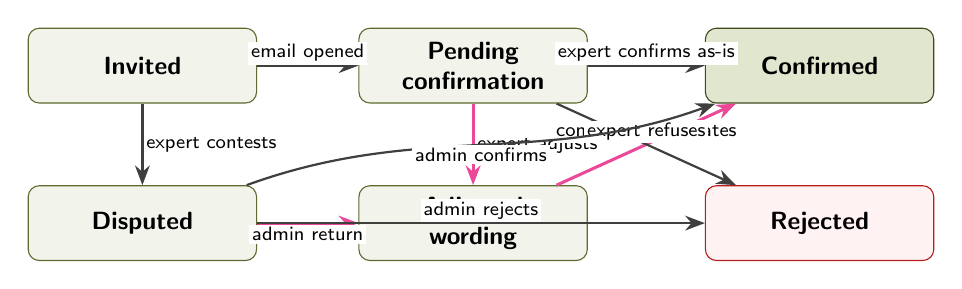
\begin{tikzpicture}[
  st/.style={draw=mil500, fill=mil50, rounded corners=4pt, minimum width=2.9cm,
    minimum height=0.95cm, align=center, font=\small\bfseries},
  good/.style={draw=mil700, fill=mil100, rounded corners=4pt, minimum width=2.9cm,
    minimum height=0.95cm, align=center, font=\small\bfseries},
  bad/.style={draw=okred, fill=red!5, rounded corners=4pt, minimum width=2.9cm,
    minimum height=0.95cm, align=center, font=\small\bfseries},
  arr/.style={-{Stealth[length=2.5mm]}, draw=char700, line width=0.8pt},
  hot/.style={-{Stealth[length=2.5mm]}, draw=acc500, line width=1.1pt},
  lab/.style={font=\scriptsize, fill=white, inner sep=1pt}
]
  \node[st] (inv) at (0,0) {Invited};
  \node[st] (pen) at (4.2,0) {Pending\\confirmation};
  \node[good] (conf) at (8.6,0) {Confirmed};
  \node[st] (adj) at (4.2,-2.0) {Adjusted\\wording};
  \node[bad] (rej) at (8.6,-2.0) {Rejected};
  \node[st] (dis) at (0,-2.0) {Disputed};

  \draw[arr] (inv) -- node[above,lab]{email opened} (pen);
  \draw[arr] (pen) -- node[above,lab]{expert confirms as-is} (conf);
  \draw[hot] (pen) -- node[right,lab]{expert adjusts} (adj);
  \draw[hot] (adj) -- node[above,lab]{company re-validates} (conf);
  \draw[arr] (pen) -- node[above,lab]{expert refuses} (rej);
  \draw[arr] (inv) -- node[right,lab]{expert contests} (dis);
  \draw[hot] (dis) -- node[below,lab]{admin return} (adj);
  \draw[arr] (dis) to[out=20,in=200] node[below,lab]{admin confirms} (conf);
  \draw[arr] (dis) -- node[above,lab]{admin rejects} (rej);
\end{tikzpicture}
\end{center}

\subsection{Transitions and services}

All transitions live in \texttt{certification/services.py} so the rules remain
in one auditable place.

\begin{center}
\begingroup\let\texttt\splittt
\small
\renewcommand{\arraystretch}{1.3}
\begin{tabularx}{\textwidth}{@{}L{4.9cm}L{3.2cm}Y@{}}
  \toprule
  \tablehead{\theadcell{Service} & \theadcell{Allowed actor} & \theadcell{Effect}} \\
  \midrule
  \texttt{declare\_contributor} & Project owner & Creates the declaration,
  auto-links an existing account by email, refuses self-declaration outside the
  publisher exception. \\
  \tablealt
  \texttt{notify\_contribution} & System & Registered expert: internal
  notification; unknown email: one active magic-link invitation. \\
  \texttt{confirm\_as\_is} & Named expert & \texttt{pending} $\rightarrow$
  \texttt{confirmed}; sends a certification email to the company. \\
  \tablealt
  \texttt{adjust\_contribution} & Named expert & Saves the corrected wording,
  flags company re-validation, notifies the company. \\
  \texttt{approve\_adjustment} & Declaring company & Confirms the adjusted
  wording; refused if no adjustment is pending. \\
  \tablealt
  \texttt{reject\_contribution} & Named expert & \texttt{rejected}, terminal,
  reason recorded. \\
  \texttt{dispute\_contribution} & Named expert & \texttt{disputed}; reason is
  mandatory and the flow freezes until arbitration. \\
  \tablealt
  \texttt{resolve\_dispute} & Staff/superuser & Confirms, rejects or returns to
  the expert. The only human intervention in the flow. \\
  \texttt{request\_client\_confirmation} & Project owner & Issues a one-time
  token to the client/master of works for an individual consultant (T1). \\
  \tablealt
  \texttt{confirm\_by\_client} & Token holder & Unauthenticated one-time
  confirmation; the token is revoked on use. \\
  \texttt{send\_invitation\_reminder} & Scheduled task & Sends a reminder,
  capped at two per invitation. \\
  \tablealt
  \texttt{expire\_stale\_invitations} & Scheduled task & Marks overdue
  invitations \texttt{expired} and keeps the audit trail. \\
  \bottomrule
\end{tabularx}
\endgroup
\end{center}

\subsection{Integrity and edge cases}

\begin{itemize}[leftmargin=1.4em,itemsep=3pt]
  \item \textbf{No self-certification.} A physical person cannot be both the
        declarant and the confirmer of the same contribution. The only
        exception is the publishing user, whose project-lead contribution is
        auto-confirmed at publish time.
  \item \textbf{Uniqueness.} A given email can only hold one contribution per
        project and role.
  \item \textbf{Confirmation timestamp.} A database constraint requires a
        \texttt{confirmed\_at} value whenever the status is \texttt{confirmed}.
  \item \textbf{Immutability.} On a confirmed contribution, the protected
        fields (project, expert, role, bullets, invited email) are frozen.
        Changing one requires leaving the confirmed state, i.e.\ starting a new
        cycle.
  \item \textbf{Adjustment loop.} An adjusted contribution returns to
        \texttt{pending\_confirmation} with
        \texttt{pending\_company\_validation=True}; the company cannot certify
        without an actual expert adjustment.
  \item \textbf{Expiry.} When reminders are exhausted and the expiration date
        passes, the invitation becomes \texttt{expired}; the historical
        contribution remains visible in the audit trail. The expert can still
        act on a live invitation through the magic link.
  \item \textbf{Confidentiality.} A private project does not expose its
        description, deliverables or media on the public proof page; only the
        certified facts (name, client, dates, contributors) are shown.
\end{itemize}

\begin{accentbox}
\textbf{Why this design matters.} The company can declare, but cannot certify.
The expert can certify, but only for themselves. The administrator can
arbitrate, but only on a dispute. No single actor can unilaterally create
certified experience: which is precisely what makes the badge meaningful.
\end{accentbox}

% =====================================================================
\section{Architecture and technical design}
\label{sec:architecture}
% =====================================================================

\subsection{Architectural style}

Urban Track is a \textbf{modular monolith}: a single Django project composed of
cohesive applications with explicit service layers. This choice keeps
transactional integrity and operational simplicity while leaving clear seams
for future extraction or external connectors.

\begin{center}
\renewcommand{\arraystretch}{1.3}
\begin{tabularx}{\textwidth}{@{}L{3.3cm}Y@{}}
  \toprule
  \tablehead{\theadcell{Concern} & \theadcell{Decision}} \\
  \midrule
  Backend & Python 3.12, Django 6.1, Django REST Framework installed for the
  API-first intent. \\
  \tablealt
  Database & SQLite, by explicit project decision. Strong relational integrity
  is enforced at the ORM and database-constraint level. \\
  Frontend & Django templates with a vendored Tailwind CSS browser build
  (pinned), configured inline; no Node/npm pipeline and no external CDN. \\
  \tablealt
  Scheduled work & Synchronous management commands, cron-triggerable. No Celery
  and no Redis, by project decision. \\
  Email & Branded HTML + plain-text emails; console backend in development,
  SMTP relay (SendGrid) configured through environment variables. \\
  \tablealt
  PDF / Word & WeasyPrint for PDF; python-docx for editable Word exports. \\
  Static files & WhiteNoise with a compressed, manifest-hashed storage backend
  in production. \\
  \bottomrule
\end{tabularx}
\end{center}

\subsection{Module dependencies}

\begin{center}
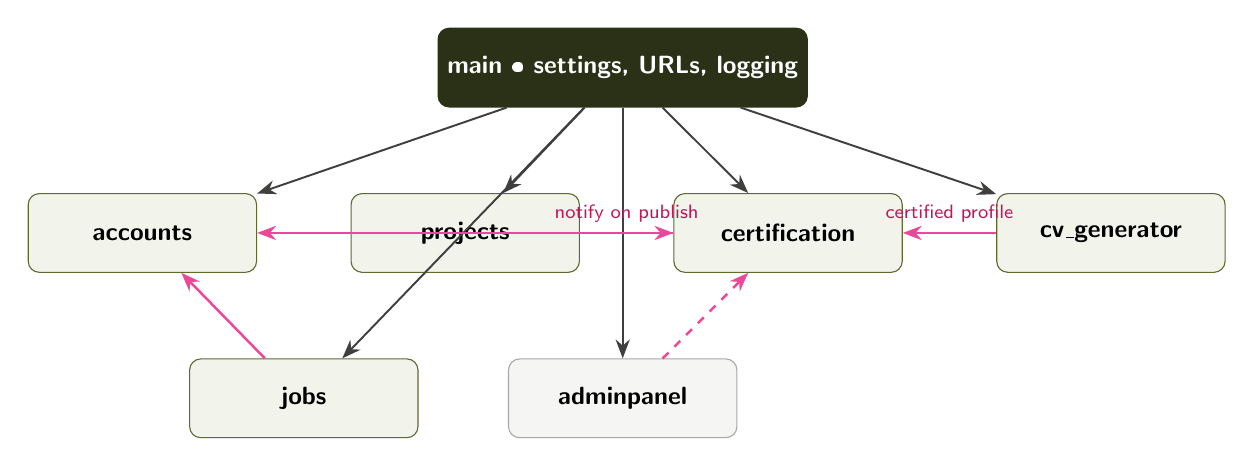
\begin{tikzpicture}[
  core/.style={draw=mil900, fill=mil900, text=white, rounded corners=4pt,
    minimum width=4.2cm, minimum height=1.0cm, align=center, font=\small\bfseries},
  app/.style={draw=mil500, fill=mil50, rounded corners=4pt,
    minimum width=2.9cm, minimum height=1.0cm, align=center, font=\small\bfseries},
  side/.style={draw=char300, fill=char50, rounded corners=4pt,
    minimum width=2.9cm, minimum height=1.0cm, align=center, font=\small\bfseries},
  arr/.style={-{Stealth[length=2.4mm]}, draw=char700, line width=0.7pt},
  dep/.style={-{Stealth[length=2.4mm]}, draw=acc500, line width=0.9pt}
]
  \node[core] (main) at (0,0) {main \textbullet\ settings, URLs, logging};
  \node[app] (accounts) at (-6.1,-2.1) {accounts};
  \node[app] (projects) at (-2.0,-2.1) {projects};
  \node[app] (cert) at (2.1,-2.1) {certification};
  \node[app] (cv) at (6.2,-2.1) {cv\_generator};
  \node[app] (jobs) at (-4.05,-4.2) {jobs};
  \node[side] (admin) at (0.0,-4.2) {adminpanel};

  \foreach \x in {accounts,projects,cert,cv,jobs,admin}{
    \draw[arr] (main) -- (\x);
  }
  \draw[dep] (projects) -- node[above,font=\scriptsize,text=acc700]{notify on publish} (cert);
  \draw[dep] (cert) -- (accounts);
  \draw[dep] (cv) -- node[above,font=\scriptsize,text=acc700]{certified profile} (cert);
  \draw[dep] (jobs) -- (accounts);
  \draw[dep, dashed] (admin) -- (cert);
\end{tikzpicture}
\end{center}

\begin{notebox}
\textbf{Dependency rule.} Dependencies flow through service functions, not
through cross-app model manipulation. \texttt{projects.services.publish\_project}
calls \texttt{certification.services.notify\_contributions\_for\_project};
\texttt{cv\_generator} reads confirmed contributions through
\texttt{ExpertProfile.confirmed\_contributions()}. This keeps each app testable
in isolation.
\end{notebox}

\subsection{Request lifecycle}

Every HTTP request passes through the following middleware chain, in order:

\begin{enumerate}[leftmargin=1.8em,itemsep=2pt]
  \item Django security middleware (headers, HTTPS redirects when configured);
  \item WhiteNoise for static files;
  \item sessions, common middleware and CSRF protection;
  \item authentication and messages;
  \item clickjacking protection;
  \item \texttt{accounts.middleware.RequireEmailConfirmationMiddleware}, which
        restricts unconfirmed accounts to the confirmation flow;
  \item \texttt{main.middleware.RequestLogMiddleware}, which assigns a
        correlation id, logs method/path/status/duration/user/IP, returns the id
        in the \texttt{X-Request-ID} response header and propagates it to every
        log line.
\end{enumerate}

\subsection{Service layer}

Business logic is not written in views. The following service modules are the
authoritative implementation of the domain rules:

\begin{center}
\begingroup\let\texttt\splittt
\small
\renewcommand{\arraystretch}{1.25}
\begin{tabularx}{\textwidth}{@{}L{5.0cm}Y@{}}
  \toprule
  \tablehead{\theadcell{Service module} & \theadcell{Responsibilities}} \\
  \midrule
  \texttt{certification.services} & Declarations, invitations, confirmations,
  adjustments, rejections, disputes, arbitration, reminders, expiry. \\
  \tablealt
  \texttt{projects.services} & Publishing, archiving, owner contribution,
  invitation dispatch. \\
  \texttt{jobs.services} & Applications, decisions, closing, deadline
  reminders. \\
  \tablealt
  \texttt{accounts.email\_confirmation} & Code issuance, confirmation, expiry,
  purge of unconfirmed accounts. \\
  \texttt{main.emails} & Absolute URL building and branded email rendering. \\
  \tablealt
  \texttt{main.logging} & Request correlation, JSON formatting and the
  \texttt{audit()} event helper. \\
  \bottomrule
\end{tabularx}
\endgroup
\end{center}

\subsection{Design system}

The website's visual identity is part of the delivery. Tokens and reusable
component classes live in \texttt{templates/base.html}:

\begin{center}
\renewcommand{\arraystretch}{1.3}
\begin{tabularx}{\textwidth}{@{}L{3.3cm}L{2.4cm}Y@{}}
  \toprule
  \tablehead{\theadcell{Token} & \theadcell{Value} & \theadcell{Usage}} \\
  \midrule
  \texttt{military} & \texttt{\#5C6B2F} & Headers, navigation, primary
  buttons, certified badges (dominant colour). \\
  \tablealt
  \texttt{accent} & \texttt{\#EC4899} & Calls to action, confirm actions,
  pending badges, used sparingly. \\
  \texttt{charcoal} & \texttt{\#1C1C1B} & Body text and footer. \\
  \tablealt
  Surfaces & \texttt{white}, \texttt{military-50} & Cards, forms, alternate
  sections. \\
  \bottomrule
\end{tabularx}
\end{center}

Reusable classes include \texttt{.btn-primary}, \texttt{.btn-accent},
\texttt{.btn-outline}, \texttt{.card}, \texttt{.card-project},
\texttt{.card-expert}, \texttt{.badge-certified}, \texttt{.badge-pending},
\texttt{.badge-rejected} and the form system (\texttt{.form-label},
\texttt{.form-input}, \texttt{.form-help}, \texttt{.form-error}). The root
\texttt{color-scheme: light} prevents OS dark mode from inverting form controls.

\subsection{Email infrastructure}

Every service that sends email goes through
\texttt{main.emails.send\_branded\_mail}, which renders a branded HTML template
plus a plain-text fallback. Links are always absolute and rooted at
\texttt{SITE\_BASE\_URL}. The delivered email templates cover:

\begin{itemize}[leftmargin=1.4em,itemsep=2pt]
  \item account confirmation code;
  \item expert invitation, reminder, registered-expert notification;
  \item company certification notice and adjustment re-validation request;
  \item client counter-signature request;
  \item job application received, new application, decision, deadline reminders
        for experts and companies;
  \item password reset.
\end{itemize}

% =====================================================================
\section{Data model}
\label{sec:data}
% =====================================================================

\subsection{Model inventory}

The delivered system defines \textbf{22 models} across four domain groups.

\begingroup\let\texttt\splittt
\small
\renewcommand{\arraystretch}{1.25}
\begin{longtable}{@{}L{3.6cm}L{4.2cm}L{7.7cm}@{}}
  \toprule
  \tablehead{\theadcell{Model} & \theadcell{Purpose} & \theadcell{Key relationships / notes}} \\
  \midrule
  \endfirsthead
  \toprule
  \tablehead{\theadcell{Model} & \theadcell{Purpose} & \theadcell{Key relationships / notes}} \\
  \midrule
  \endhead
  \bottomrule
  \endlastfoot
  \multicolumn{3}{@{}l}{\color{mil700}\textbf{Accounts and identity}}\\
  \midrule
  \texttt{User} & Custom account & Unique email, role, company, avatar,
  permanent \texttt{OX-XXXXXX}, email-confirmation fields. \\
  \texttt{Company} & Organisation & Unique name, public profile, membership
  helpers. \\
  \texttt{CompanyMembership} & Affiliation lifecycle & User + company, status,
  role, requester/reviewer audit trail; unique per pair. \\
  \texttt{Skill} & Skill tag & Many-to-many with profiles. \\
  \texttt{ExpertProfile} & Public portfolio & One-to-one with user; headline,
  bio, location, strengths, languages, CV template preference. \\
  \texttt{Training} & Education entry & FK to profile. \\
  \texttt{Position} & Professional position & FK to profile; declared, not
  certifying. \\
  \texttt{Mandate} & Association mandate & FK to profile. \\
  \texttt{Publication} & Publication reference & FK to profile. \\
  \texttt{TeachingEntry} & Teaching activity & FK to profile. \\
  \texttt{MediaAppearance} & Media appearance & FK to profile; title, outlet,
  year, URL. \\
  \midrule
  \multicolumn{3}{@{}l}{\color{mil700}\textbf{Projects and referentials}}\\
  \midrule
  \texttt{Country} & Structured country & Unique name and optional ISO-3 code. \\
  \texttt{Funder} & Financing institution & Distinct from the client. \\
  \texttt{Client} & Client / master of works & Structured referential. \\
  \texttt{ProjectTag} & Thematic keyword & Shared across projects for filtering. \\
  \texttt{Project} & Published project & Owner, lifecycle, visibility,
  donor-format fields, dates, budget, client; duration constraints. \\
  \texttt{ProjectLink} & External reference & Label + URL. \\
  \texttt{ProjectMedia} & Optional media & Image or document, caption, upload
  date. \\
  \midrule
  \multicolumn{3}{@{}l}{\color{mil700}\textbf{Certification}}\\
  \midrule
  \texttt{ProjectContribution} & Declared contribution & Project + expert/email,
  role, bullets, status, confirmation source, one-time client token; unique
  project/email/role; confirmed timestamp constraint. \\
  \texttt{ExpertInvitation} & Magic-link invitation & Contribution, email,
  UUID token, expiry, status, reminder count. \\
  \midrule
  \multicolumn{3}{@{}l}{\color{mil700}\textbf{Jobs}}\\
  \midrule
  \texttt{Job} & Job offer & Publisher, location, contract type, description,
  requirements, compensation, deadline, status. \\
  \texttt{JobApplication} & Application & Job + applicant, cover letter,
  status, timestamps; unique per job/applicant. \\
\end{longtable}
\endgroup
\normalsize

\subsection{Key constraints}

\begin{itemize}[leftmargin=1.4em,itemsep=3pt]
  \item \texttt{User.professional\_id} is unique and generated once.
  \item \texttt{User.email} is unique; emails are normalised before save.
  \item \texttt{CompanyMembership} is unique per (user, company).
  \item \texttt{ProjectContribution} is unique per (project, invited email,
        role), and a confirmed contribution must carry \texttt{confirmed\_at}.
  \item \texttt{JobApplication} is unique per (job, applicant).
  \item Project duration must end on or after its start; the personal
        participation window follows the same rule.
\end{itemize}

\subsection{Data lifecycle}

\begin{itemize}[leftmargin=1.4em,itemsep=3pt]
  \item \textbf{Unconfirmed accounts} are deleted after the 24-hour
        confirmation window by the scheduled purge command
        (\texttt{purge\_unconfirmed}).
  \item \textbf{Invitations} expire after about 14 days; reminders are capped at
        two.
  \item \textbf{Draft projects} can be deleted. Published projects cannot: they
        must be archived so their certified history survives.
  \item \textbf{Certified contributions} are never deleted through the normal
        flow; disputes and arbitration are recorded as audit events.
\end{itemize}

% =====================================================================
\section{Security, privacy and auditability}
\label{sec:security}
% =====================================================================

\subsection{Authentication and account protection}

\begin{itemize}[leftmargin=1.4em,itemsep=3pt]
  \item Django authentication with a custom user model; login by email or
        username.
  \item Password validators: minimum length 8, similarity check, common-password
        check and numeric-only check.
  \item Six-digit email confirmation code, valid 24 hours, required before the
        account can use the platform (\texttt{RequireEmailConfirmationMiddleware}).
  \item Secure password-reset tokens; password change requires the current
        password.
  \item Email changes re-enter the confirmation flow.
\end{itemize}

\subsection{Authorization}

\begin{itemize}[leftmargin=1.4em,itemsep=3pt]
  \item Project management is restricted to the publishing user (or
        superuser); contribution validation is restricted to the declaring
        company.
  \item Contribution actions are restricted to the named expert; sequential
        primary keys cannot be used to act on someone else's contribution.
  \item Job decisions and closing are restricted to the offer publisher.
  \item The system-admin console is restricted to nominated administrators and
        superusers.
  \item Company membership approval is restricted to approved company
        administrators.
\end{itemize}

\subsection{Data protection and privacy}

\begin{itemize}[leftmargin=1.4em,itemsep=3pt]
  \item Personal data is optional and minimised: birth date, phone and
        nationality are optional; birth date is explicitly kept confidential
        and never shown on the public site.
  \item Public profiles display only confirmed contributions as certified
        experience; self-declared content is labelled as such.
  \item Private projects expose only a minimal proof page when a certified
        contribution exists; description, deliverables and media stay private.
  \item Audit events log identifiers, never secrets or personal data.
\end{itemize}

\subsection{Application security}

\begin{itemize}[leftmargin=1.4em,itemsep=3pt]
  \item CSRF protection on all state-changing forms; clickjacking protection.
  \item Template auto-escaping prevents HTML injection; the ORM prevents SQL
        injection.
  \item Uploaded files are validated by forms and stored under dedicated media
        paths.
  \item Secrets and provider credentials are read from environment variables;
        no secret is committed to the repository.
  \item \texttt{SECURE\_PROXY\_SSL\_HEADER} makes Django trust the reverse
        proxy's HTTPS indication, so reset and confirmation links use HTTPS.
  \item One-time UUID tokens protect magic links and client confirmation; the
        client token is revoked on use.
  \item Dependency auditing is part of CI (\texttt{pip-audit}); recent commits
        patched known vulnerabilities.
\end{itemize}

\subsection{Logging and audit trail}

\begin{itemize}[leftmargin=1.4em,itemsep=3pt]
  \item Every request is logged with a correlation id returned in
        \texttt{X-Request-ID}; the id is attached to all log lines emitted while
        handling the request.
  \item Logs go to stdout (captured by systemd/journald) and, outside tests, to
        rotating files \texttt{logs/urbantrack.log} and \texttt{logs/errors.log}.
  \item \texttt{LOG\_FORMAT=json} produces one JSON object per line for log
        collectors; \texttt{LOG\_LEVEL}, \texttt{LOG\_DIR},
        \texttt{LOG\_MAX\_BYTES}, \texttt{LOG\_BACKUP\_COUNT} and
        \texttt{LOG\_SKIP\_PATHS} are environment-tunable.
  \item Business events are written to the \texttt{urbantrack.audit} logger:
        project publishing/archiving, contribution declaration, confirmation,
        adjustment, rejection, dispute and arbitration, invitation and reminder,
        membership lifecycle, job application and decision, sign-up, login,
        email confirmation and account purge.
\end{itemize}

% =====================================================================
\section{Quality assurance}
\label{sec:qa}
% =====================================================================

\subsection{Automated test suite}

The delivered test suite contains \textbf{288 passing tests}, executed in about
26 seconds with an in-memory test database.

\begin{center}
\renewcommand{\arraystretch}{1.3}
\begin{tabularx}{\textwidth}{@{}L{4.0cm}L{2.2cm}Y@{}}
  \toprule
  \tablehead{\theadcell{Module} & \theadcell{Tests} & \theadcell{Coverage focus}} \\
  \midrule
  \texttt{accounts} & 90 & Identity, OX-ID, confirmation, memberships,
  portfolio, public profiles, settings. \\
  \tablealt
  \texttt{certification} & 64 & State machine, invitations, adjustments,
  disputes, client confirmation, review routes. \\
  \texttt{projects} & 58 & Lifecycle, publishing, referentials, visibility,
  proof pages, media. \\
  \tablealt
  \texttt{cv\_generator} & 34 & Context contracts, labels, completeness,
  exports, demo data. \\
  \texttt{jobs} & 18 & Offers, applications, decisions, reminders. \\
  \tablealt
  \texttt{adminpanel} & 15 & Access control and administrative operations. \\
  \texttt{main} & 9 & Logging, middleware, error handlers, email helpers. \\
  \midrule
  \textbf{Total} & \textbf{288} & Full platform, including edge cases and permissions. \\
  \bottomrule
\end{tabularx}
\end{center}

\subsection{Continuous integration}

Every push to \texttt{main} and every pull request runs three jobs:

\begin{enumerate}[leftmargin=1.8em,itemsep=3pt]
  \item \textbf{Lint}: \texttt{ruff check .} and
        \texttt{ruff format --check .}.
  \item \textbf{Security}: \texttt{pip-audit -r requirements.txt}.
  \item \textbf{Tests}: \texttt{manage.py check}, missing-migration
        detection, static collection, full test suite and
        \texttt{coverage report --fail-under=80}.
\end{enumerate}

\begin{keybox}
\textbf{Quality gate.} A change cannot be delivered if lint fails, a dependency
has a known vulnerability, a migration is missing, a test fails, or coverage
drops below 80\%.
\end{keybox}

\subsection{Testing strategy}

\begin{itemize}[leftmargin=1.4em,itemsep=3pt]
  \item \textbf{Domain-first}: service transitions are tested independently of
        the views, including invalid transitions and permission failures.
  \item \textbf{Workflow scenarios}: full paths from declaration to certified
        contribution and from application to decision.
  \item \textbf{Edge cases}: self-declaration, duplicate emails, expired codes,
        exhausted reminders, withdrawn applications, private proof pages.
  \item \textbf{Contracts}: CV template contexts are validated against explicit
        data contracts.
  \item \textbf{Presentation}: key pages and access rules are exercised through
        the Django test client.
\end{itemize}

% =====================================================================
\section{Deployment and operations}
\label{sec:ops}
% =====================================================================

\subsection{Environments}

\begin{center}
\renewcommand{\arraystretch}{1.35}
\begin{tabularx}{\textwidth}{@{}L{3.1cm}Y@{}}
  \toprule
  \tablehead{\theadcell{Environment} & \theadcell{Setup}} \\
  \midrule
  \textbf{Development} & \texttt{runserver}, SQLite, console email backend,
  local media, rotating logs. \\
  \tablealt
  \textbf{Production} & Ubuntu VPS, Gunicorn (3 workers) on a Unix socket,
  systemd service, nginx reverse proxy with TLS, WhiteNoise for static files,
  SMTP relay for email, cron for scheduled commands. \\
  \bottomrule
\end{tabularx}
\end{center}

\subsection{Production topology}

\begin{center}
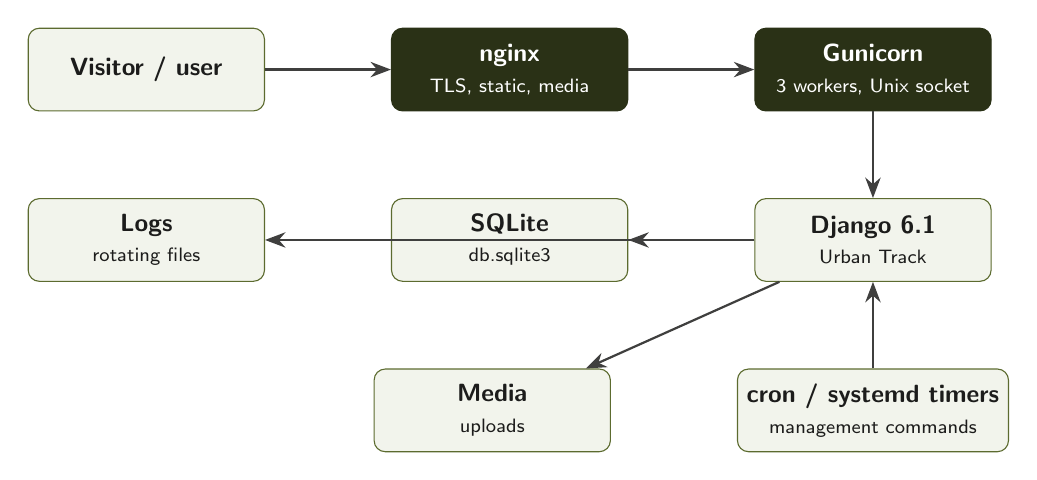
\begin{tikzpicture}[
  box/.style={draw=mil500, fill=mil50, rounded corners=4pt, minimum width=3.0cm,
    minimum height=1.05cm, align=center, font=\small\bfseries, text=char900},
  edge/.style={draw=mil900, fill=mil900, text=white, rounded corners=4pt,
    minimum width=3.0cm, minimum height=1.05cm, align=center, font=\small\bfseries},
  arr/.style={-{Stealth[length=2.6mm]}, draw=char700, line width=0.8pt}
]
  \node[box] (client) {Visitor / user};
  \node[edge, right=1.6cm of client] (proxy) {nginx\\{\scriptsize\mdseries TLS, static, media}};
  \node[edge, right=1.6cm of proxy] (gunicorn) {Gunicorn\\{\scriptsize\mdseries 3 workers, Unix socket}};
  \node[box, below=1.1cm of gunicorn] (django) {Django 6.1\\{\scriptsize\mdseries Urban Track}};
  \node[box, left=1.6cm of django] (sqlite) {SQLite\\{\scriptsize\mdseries db.sqlite3}};
  \node[box, left=1.6cm of sqlite] (logs) {Logs\\{\scriptsize\mdseries rotating files}};
  \node[box, below=1.1cm of django] (cron) {cron / systemd timers\\{\scriptsize\mdseries management commands}};
  \node[box, left=1.6cm of cron] (media) {Media\\{\scriptsize\mdseries uploads}};
  \draw[arr] (client) -- (proxy);
  \draw[arr] (proxy) -- (gunicorn);
  \draw[arr] (gunicorn) -- (django);
  \draw[arr] (django) -- (sqlite);
  \draw[arr] (django) -- (logs);
  \draw[arr] (cron) -- (django);
  \draw[arr] (django) -- (media);
\end{tikzpicture}
\end{center}

\subsection{Deployment pipeline}

A push to \texttt{main} triggers the deploy workflow:

\begin{enumerate}[leftmargin=1.8em,itemsep=3pt]
  \item checkout and full test run on GitHub Actions;
  \item SSH connection to the VPS using a dedicated deploy key;
  \item \texttt{git fetch origin main} and \texttt{git reset --hard origin/main};
  \item virtual-environment self-healing and dependency installation;
  \item installation of PDF system libraries (Pango, Cairo, GdkPixbuf);
  \item \texttt{manage.py migrate} and \texttt{manage.py collectstatic};
  \item restart of the \texttt{UrbanTrack.service} systemd unit;
  \item service health check (\texttt{systemctl is-active}).
\end{enumerate}

\subsection{Scheduled tasks}

\begin{center}
\renewcommand{\arraystretch}{1.3}
\begin{tabularx}{\textwidth}{@{}L{5.2cm}Y@{}}
  \toprule
  \tablehead{\theadcell{Command} & \theadcell{Purpose}} \\
  \midrule
  \texttt{process\_invitations} & Sends due invitation reminders (capped at
  two) and expires overdue invitations. \\
  \tablealt
  \texttt{process\_jobs} & Sends deadline reminders to applicants and
  companies (default horizon: 3 days; \texttt{--days} option). \\
  \texttt{purge\_unconfirmed} & Deletes accounts still unconfirmed after the
  24-hour window. \\
  \tablealt
  \texttt{seed\_demo\_expert} & Creates an idempotent, fully populated demo
  expert with certified projects. \\
  \bottomrule
\end{tabularx}
\end{center}

Example cron entries:

\begin{lstlisting}[language=bash]
# Certification reminders and expiry
0 8 * * * cd /home/ubuntu/UrbanTrack && env/bin/python manage.py process_invitations

# Job deadline reminders
0 9 * * * cd /home/ubuntu/UrbanTrack && env/bin/python manage.py process_jobs

# Purge abandoned sign-ups
30 3 * * * cd /home/ubuntu/UrbanTrack && env/bin/python manage.py purge_unconfirmed
\end{lstlisting}

\subsection{Configuration}

Settings are environment-driven through \texttt{.env} (loaded in development)
and real environment variables (which always take precedence). Key variables
are listed in Appendix~\ref{app:env}. Notable defaults:

\begin{itemize}[leftmargin=1.4em,itemsep=2pt]
  \item invitation expiry: 14 days; reminder threshold: 5 days; maximum two
        reminders;
  \item confirmation code: 6 digits, 24 hours;
  \item default email backend: console;
  \item default logging level: \texttt{INFO}, text format;
  \item static files: WhiteNoise compressed manifest storage;
  \item database: \texttt{db.sqlite3}, configurable via \texttt{SQLITE\_DB\_NAME}.
\end{itemize}

\subsection{Backup and recovery considerations}

The production data lives in the SQLite database file and the
\texttt{media/} directory. A robust operational routine should snapshot both
together and keep copies off the VPS. Because SQLite is a single file, backups
are simple, but they must be taken consistently (for example with the SQLite
online backup API or after a short maintenance stop) and restore procedures
should be rehearsed. No health or version endpoint is exposed, by explicit
client decision.

% =====================================================================
\section{Delivery status and roadmap}
\label{sec:status}
% =====================================================================

\subsection{Delivered epics}

\begin{center}
\renewcommand{\arraystretch}{1.3}
\begin{tabularx}{\textwidth}{@{}L{1.3cm}L{9.3cm}L{2.4cm}@{}}
  \toprule
  \tablehead{\theadcell{Epic} & \theadcell{Scope} & \theadcell{Status}} \\
  \midrule
  -1 & Bootstrap: repository, applications, SQLite, Tailwind JS, custom user,
  OX-ID, CI. & \delivered \\
  \tablealt
  0 & Design system and UI foundations: tokens, components, badges, profile
  typography. & \delivered \\
  1 & Core data models, cross-confirmation state machine, integrity constraints. & \delivered \\
  \tablealt
  2 & Project publishing screens: create, declare contributors, publish,
  archive. & \delivered \\
  3 & Expert invitation and landing: magic link, inline account creation. & \delivered \\
  \tablealt
  4 & Certification and public profiles: directory, project pages, cross-links,
  trust score. & \delivered \\
  5 & Edge cases: reminders/expiry command, disputes, admin arbitration. & \delivered \\
  \tablealt
  6 & Email infrastructure: branded templates and console backend. Provider
  integration and open/click tracking remain. & \delivered \\
  7 & Multi-template CV generator: AFD and World Bank, FR/EN, PDF/Word,
  portfolio self-edit. & \delivered \\
  \tablealt
  8 & Job board: publish, apply, accept/decline notifications, deadline
  reminders. & \delivered \\
  9 & External connectors: World Bank API, AFD API. & \planned \\
  \tablealt
  10 & AI matchmaking and success prediction. & \planned \\
  \bottomrule
\end{tabularx}
\end{center}

\subsection{Explicit client decisions}

The following decisions intentionally override the original generic
specification and are part of the delivered architecture:

\begin{itemize}[leftmargin=1.4em,itemsep=3pt]
  \item \textbf{SQLite instead of PostgreSQL}; no database server to operate.
  \item \textbf{No Celery and no Redis}; scheduled work runs as synchronous
        management commands.
  \item \textbf{Tailwind browser build instead of an npm pipeline}; no Node.js
        toolchain, no external CDN.
  \item \textbf{No health or versioned endpoints}; operational checks rely on
        the process manager and logs.
  \item \textbf{SendGrid} retained as the transactional email provider;
        development uses the console backend.
\end{itemize}

\subsection{Flagged additive fields}

None of the mandated data-model fields was altered. The following additive
fields were required by the business rules and are documented as deliberate
deviations-by-addition:

\begin{itemize}[leftmargin=1.4em,itemsep=3pt]
  \item \texttt{Project.published\_by}: ownership of the publishing company user.
  \item \texttt{ProjectContribution.pending\_company\_validation}: distinguishes
        ``awaiting the expert's first answer'' from ``the company must
        re-validate an adjusted wording''.
  \item \texttt{ProjectContribution.rejection\_reason} and
        \texttt{dispute\_reason}: audit trail for arbitration.
  \item \texttt{ExpertProfile.cv\_template}: per-expert CV skin preference.
\end{itemize}

\subsection{Recommended next steps}

\begin{enumerate}[leftmargin=1.8em,itemsep=3pt]
  \item Connect the SendGrid provider and implement open/click webhooks
        (completion of Epic 6).
  \item Implement the World Bank and AFD connectors (Epic 9).
  \item Prepare AI matchmaking on certified data (Epic 10).
  \item Add an operational backup and restore runbook for the SQLite database
        and media directory.
  \item Consider PostgreSQL when concurrent write volume justifies it; the ORM
        layer keeps the migration path straightforward.
\end{enumerate}

% =====================================================================
\section{Getting started}
\label{sec:start}
% =====================================================================

\subsection{Prerequisites}

\begin{itemize}[leftmargin=1.4em,itemsep=2pt]
  \item Python 3.12;
  \item the system libraries required by WeasyPrint (Pango, Cairo, GdkPixbuf);
  \item on the VPS: Gunicorn, nginx, systemd and a virtual environment.
\end{itemize}

\subsection{Local installation}

\begin{lstlisting}[language=bash]
python3.12 -m venv env
source env/bin/activate
pip install -r requirements.txt

cp .env.example .env        # adjust values if needed
python manage.py migrate
python manage.py runserver  # http://127.0.0.1:8000/
\end{lstlisting}

Create an administrator account, then open \texttt{/admin/}:

\begin{lstlisting}[language=bash]
python manage.py createsuperuser
\end{lstlisting}

Load a fully populated demo expert (idempotent):

\begin{lstlisting}[language=bash]
python manage.py seed_demo_expert
\end{lstlisting}

Demo credentials: \texttt{aminata.sow@demo.urbantrack} /
\texttt{Demo!Expert2025}.

\subsection{Tests and lint}

\begin{lstlisting}[language=bash]
python manage.py test        # 288 tests
ruff check .                 # lint (line length 100)
ruff format --check .        # formatting
\end{lstlisting}

\subsection{Project layout}

\begin{lstlisting}
main/            Django project: settings, URLs, logging, middleware, email
accounts/        identity, OX-ID, confirmation, memberships, portfolios
projects/        project lifecycle, referentials, media, public proof pages
certification/   contributions, invitations, state machine, arbitration
cv_generator/    multi-skin CV context, FR/EN labels, PDF and Word exports
jobs/            offers, applications, decisions, deadline reminders
adminpanel/      system-administration console
templates/       base shell, design system, public pages, emails
static/          vendored Tailwind build, logos, free-licence photos
docs/            specifications, CV labels dictionary, this documentation
.github/          CI and deployment workflows
\end{lstlisting}

% =====================================================================
\appendix
% =====================================================================

\section{Application route map}
\label{app:routes}

\begin{center}
\renewcommand{\arraystretch}{1.2}
\begin{longtable}{@{}L{5.8cm}L{3.2cm}L{6.4cm}@{}}
  \toprule
  \tablehead{\theadcell{Path} & \theadcell{Name} & \theadcell{Access}} \\
  \midrule
  \endfirsthead
  \toprule
  \tablehead{\theadcell{Path} & \theadcell{Name} & \theadcell{Access}} \\
  \midrule
  \endhead
  \bottomrule
  \endlastfoot
  \texttt{/\allowbreak } & \texttt{home} & Public \\
  \texttt{/\allowbreak about/\allowbreak } & \texttt{about} & Public \\
  \texttt{/\allowbreak signup/\allowbreak } & \texttt{accounts:\allowbreak signup} & Public \\
  \texttt{/\allowbreak login/\allowbreak } & \texttt{accounts:\allowbreak login} & Public \\
  \texttt{/\allowbreak logout/\allowbreak } & \texttt{accounts:\allowbreak logout} & Authenticated \\
  \texttt{/\allowbreak confirm-email/\allowbreak } & \texttt{accounts:\allowbreak confirm\_\allowbreak email} & Unconfirmed users \\
  \texttt{/\allowbreak password-reset/\allowbreak } & \texttt{accounts:\allowbreak password\_\allowbreak reset} & Public \\
  \texttt{/\allowbreak dashboard/\allowbreak } & \texttt{accounts:\allowbreak dashboard} & Authenticated \\
  \texttt{/\allowbreak settings/\allowbreak } & \texttt{accounts:\allowbreak settings} & Authenticated \\
  \texttt{/\allowbreak portfolio/\allowbreak edit/\allowbreak } & \texttt{accounts:\allowbreak profile\_\allowbreak edit} & Authenticated \\
  \texttt{/\allowbreak experts/\allowbreak } & \texttt{accounts:\allowbreak expert\_\allowbreak list} & Public \\
  \texttt{/\allowbreak experts/\allowbreak \textless OX-ID\textgreater\allowbreak /\allowbreak } & \texttt{accounts:\allowbreak public\_\allowbreak profile} & Public \\
  \texttt{/\allowbreak companies/\allowbreak \textless id\textgreater\allowbreak /\allowbreak } & \texttt{accounts:\allowbreak company\_\allowbreak public} & Public \\
  \texttt{/\allowbreak projects/\allowbreak } & \texttt{projects:\allowbreak list} & Public \\
  \texttt{/\allowbreak projects/\allowbreak new/\allowbreak } & \texttt{projects:\allowbreak create} & Authenticated \\
  \texttt{/\allowbreak projects/\allowbreak \textless id\textgreater\allowbreak /\allowbreak } & \texttt{projects:\allowbreak detail} & Public / proof \\
  \texttt{/\allowbreak projects/\allowbreak \textless id\textgreater\allowbreak /\allowbreak manage/\allowbreak } & \texttt{projects:\allowbreak manage} & Owner \\
  \texttt{/\allowbreak certification/\allowbreak invitations/\allowbreak \textless uuid\textgreater\allowbreak /\allowbreak } & \texttt{certification:\allowbreak invitation\_\allowbreak landing} & Magic link \\
  \texttt{/\allowbreak certification/\allowbreak contributions/\allowbreak \textless id\textgreater\allowbreak /\allowbreak review/\allowbreak } & \texttt{certification:\allowbreak contribution\_\allowbreak review} & Named expert \\
  \texttt{/\allowbreak certification/\allowbreak client-confirm/\allowbreak \textless uuid\textgreater\allowbreak /\allowbreak } & \texttt{certification:\allowbreak client\_\allowbreak confirm} & Token holder \\
  \texttt{/\allowbreak cv/\allowbreak } & \texttt{cv\_\allowbreak generator:\allowbreak builder} & Authenticated \\
  \texttt{/\allowbreak cv/\allowbreak \textless skin\textgreater\allowbreak /\allowbreak } & \texttt{cv\_\allowbreak generator:\allowbreak preview} & Authenticated \\
  \texttt{/\allowbreak cv/\allowbreak \textless skin\textgreater\allowbreak /\allowbreak pdf/\allowbreak } & \texttt{cv\_\allowbreak generator:\allowbreak pdf} & Authenticated \\
  \texttt{/\allowbreak cv/\allowbreak \textless skin\textgreater\allowbreak /\allowbreak docx/\allowbreak } & \texttt{cv\_\allowbreak generator:\allowbreak docx} & Authenticated \\
  \texttt{/\allowbreak jobs/\allowbreak } & \texttt{jobs:\allowbreak list} & Public \\
  \texttt{/\allowbreak jobs/\allowbreak new/\allowbreak } & \texttt{jobs:\allowbreak create} & Authenticated \\
  \texttt{/\allowbreak jobs/\allowbreak \textless id\textgreater\allowbreak /\allowbreak } & \texttt{jobs:\allowbreak detail} & Public \\
  \texttt{/\allowbreak jobs/\allowbreak \textless id\textgreater\allowbreak /\allowbreak apply/\allowbreak } & \texttt{jobs:\allowbreak apply} & Authenticated \\
  \texttt{/\allowbreak jobs/\allowbreak \textless id\textgreater\allowbreak /\allowbreak manage/\allowbreak } & \texttt{jobs:\allowbreak manage} & Publisher \\
  \texttt{/\allowbreak admin-panel/\allowbreak } & \texttt{adminpanel:\allowbreak dashboard} & System admin \\
  \texttt{/\allowbreak admin/\allowbreak } & Django admin & Staff \\
  \texttt{/\allowbreak api/\allowbreak } & DRF browsable API & Public surface \\
\end{longtable}
\end{center}

\section{Management commands and scheduled tasks}
\label{app:commands}

\begin{center}
\renewcommand{\arraystretch}{1.3}
\begin{tabularx}{\textwidth}{@{}L{5.2cm}Y@{}}
  \toprule
  \tablehead{\theadcell{Command} & \theadcell{Behaviour}} \\
  \midrule
  \texttt{python manage.py test} & Runs the full 288-test suite. \\
  \tablealt
  \texttt{python manage.py migrate} & Applies the 27 migrations. \\
  \texttt{python manage.py collectstatic} & Builds the WhiteNoise manifest. \\
  \tablealt
  \texttt{python manage.py process\_invitations} & Reminders and expiry. \\
  \texttt{python manage.py process\_jobs [--days N]} & Job deadline reminders. \\
  \tablealt
  \texttt{python manage.py purge\_unconfirmed} & Deletes abandoned sign-ups. \\
  \texttt{python manage.py seed\_demo\_expert} & Creates demo data. \\
  \bottomrule
\end{tabularx}
\end{center}

\section{Environment variables}
\label{app:env}

\begin{center}
\begingroup\let\texttt\splittt
\renewcommand{\arraystretch}{1.25}
\begin{longtable}{@{}L{4.3cm}L{4.4cm}L{6.3cm}@{}}
  \toprule
  \tablehead{\theadcell{Variable} & \theadcell{Default} & \theadcell{Purpose}} \\
  \midrule
  \endfirsthead
  \toprule
  \tablehead{\theadcell{Variable} & \theadcell{Default} & \theadcell{Purpose}} \\
  \midrule
  \endhead
  \bottomrule
  \endlastfoot
  \texttt{DJANGO\_SECRET\_KEY} & dev-only key & Cryptographic signing key;
  must be set in production. \\
  \texttt{DJANGO\_ALLOWED\_HOSTS} & \texttt{localhost,127.0.0.1} & Host header
  allow-list. \\
  \texttt{SQLITE\_DB\_NAME} & \texttt{db.sqlite3} & SQLite database filename. \\
  \texttt{SITE\_BASE\_URL} & \texttt{http://localhost:8000} & Absolute base URL
  used in emails. \\
  \texttt{EMAIL\_BACKEND} & console & Django email backend. \\
  \texttt{EMAIL\_HOST} & \texttt{smtp.sendgrid.net} & SMTP host. \\
  \texttt{EMAIL\_PORT} & \texttt{587} & SMTP port. \\
  \texttt{EMAIL\_HOST\_USER} & \texttt{apikey} & SMTP user (SendGrid). \\
  \texttt{EMAIL\_HOST\_PASSWORD} & empty & SMTP password / API key. \\
  \texttt{EMAIL\_USE\_TLS} / \texttt{EMAIL\_USE\_SSL} & false & Transport security. \\
  \texttt{DEFAULT\_FROM\_EMAIL} & \texttt{noreply@urbantrack.africa} & Sender address. \\
  \texttt{LOG\_LEVEL} & \texttt{INFO} & Application log level. \\
  \texttt{LOG\_FORMAT} & \texttt{text} & \texttt{text} or \texttt{json}. \\
  \texttt{LOG\_DIR} & \texttt{logs} & Log directory. \\
  \texttt{LOG\_TO\_FILE} & \texttt{True} & Enable rotating files. \\
  \texttt{LOG\_MAX\_BYTES} & \texttt{10485760} & Rotation size. \\
  \texttt{LOG\_BACKUP\_COUNT} & \texttt{5} & Number of rotated files. \\
  \texttt{LOG\_SKIP\_PATHS} & static, media, favicon & Paths excluded from access logs. \\
  \texttt{LAUNCH\_COUNTER\_THRESHOLD} & \texttt{1} & Dashboard launch-stat threshold. \\
\end{longtable}
\endgroup
\end{center}

\section{Glossary}
\label{app:glossary}

\begin{center}
\renewcommand{\arraystretch}{1.3}
\begin{tabularx}{\textwidth}{@{}L{3.4cm}Y@{}}
  \toprule
  \tablehead{\theadcell{Term} & \theadcell{Definition}} \\
  \midrule
  \textbf{Certification} & Independent cross-confirmation of a contribution by
  the named expert (or the client for an individual consultant). \\
  \tablealt
  \textbf{Contribution} & A declared role and set of achievements of one expert
  on one project. \\
  \textbf{Cross-confirmation} & The double-validation principle: the company
  declares, the expert confirms. \\
  \tablealt
  \textbf{Expert invitation} & A magic-link email sent to an unregistered
  contributor, carrying a secret UUID token with an expiry date. \\
  \textbf{Ox-ID / OX-XXXXXX} & The permanent, unique professional identifier of
  an Urban Track user. \\
  \tablealt
  \textbf{Proof page} & A minimal public project page kept accessible when a
  certified contribution must remain traceable but the project is not public. \\
  \textbf{Trust score} & A weighted sum of certified contributions (director 4,
  manager 3, specialist/consultant/engineer 2, assistant/other 1). \\
  \tablealt
  \textbf{Declared content} & Self-declared portfolio sections (positions,
  publications, teaching, etc.) that are explicitly not third-party verified. \\
  \textbf{Skin} & A CV visual template: AFD or World Bank. \\
  \tablealt
  \textbf{WeasyPrint} & The HTML-to-PDF engine used for CV export. \\
  \textbf{WhiteNoise} & The static-file server used in production without nginx. \\
  \bottomrule
\end{tabularx}
\end{center}

\vfill
\begin{center}
{\color{char300}\small End of document}\\[4pt]
{\color{mil700}\bfseries Urban Track \textbullet\ Global project documentation
\textbullet\ Final delivery \textbullet\ November 2026}
\end{center}

\end{document}
